%%%%%%%%%%%%%%%%%%%%%%%%%%%%%%%%%%%%%%%%%
% Template
% LaTeX Template
% Version 1.0 (December 8 2014)
%
% This template has been downloaded from:
% http://www.LaTeXTemplates.com
%
% Original author:
% Brandon Fryslie
% With extensive modifications by:
% Vel (vel@latextemplates.com)
%
% License:
% CC BY-NC-SA 3.0 (http://creativecommons.org/licenses/by-nc-sa/3.0/)
%
% Authors:
% Sabbir Ahmed
% 
%%%%%%%%%%%%%%%%%%%%%%%%%%%%%%%%%%%%%%%%%

\documentclass[paper=usletter, fontsize=12pt]{article}
%%%%%%%%%%%%%%%%%%%%%%%%%%%%%%%%%%%%%%%%%
% Contract Structural Definitions File Version 1.0 (December 8 2014)
%
% Created by: Vel (vel@latextemplates.com)
% 
% This file has been downloaded from: http://www.LaTeXTemplates.com
%
% License: CC BY-NC-SA 3.0 (http://creativecommons.org/licenses/by-nc-sa/3.0/)
%
%%%%%%%%%%%%%%%%%%%%%%%%%%%%%%%%%%%%%%%%%

\usepackage{geometry} % Required to modify the page layout
\usepackage{multicol}
\usepackage{amsmath}
\usepackage{amssymb}

\usepackage[pdftex]{graphicx}
\usepackage{wrapfig}
\usepackage[font=scriptsize, labelfont=bf]{caption}
\usepackage[utf8]{inputenc} % Required for including letters with accents
\usepackage[T1]{fontenc} % Use 8-bit encoding that has 256 glyphs

\usepackage{avant} % Use the Avantgarde font for headings
\usepackage{courier}
\usepackage{xparse}
\usepackage{xcolor}
\usepackage{listings}  % for code verbatim and console outputs

\setlength{\textwidth}{16cm} % Width of the text on the page
\setlength{\textheight}{23cm} % Height of the text on the page
\setlength{\oddsidemargin}{0cm} % Width of the margin - negative to move text left, positive to move it right
\setlength{\topmargin}{-1.25cm} % Reduce the top margin

\setlength{\parindent}{0mm} % Don't indent paragraphs
\setlength{\parskip}{2.5mm} % Whitespace between paragraphs
\renewcommand{\baselinestretch}{1.5}

\definecolor{green}{rgb}{0.18, 0.55, 0.34}

\graphicspath{ {figures/} }
\captionsetup[table]{skip=10pt}

\lstset{language=C, keywordstyle={\bfseries \color{black}}}

% defines algorithm counter for chapter-level
\newcounter{nalg}[section]

%defines appearance of the algorithm counter
\renewcommand{\thenalg}{\thesection .\arabic{nalg}}

% defines a new caption label as Algorithm x.y
\DeclareCaptionLabelFormat{algocaption}{Algorithm \thenalg}

% defines the algorithm listing environment
\lstnewenvironment{pseudocode}[1][] {
    \refstepcounter{nalg}  % increments algorithm number
    \captionsetup{font=normalsize, labelformat=algocaption, labelsep=colon}
    \lstset{
        breaklines=true,
        mathescape=true,
        numbers=left,
        numberstyle=\scriptsize,
        basicstyle=\footnotesize\ttfamily,
        keywordstyle=\color{black}\bfseries,
        keywords={input, output, return, parallel, function, for, to, in, if,
        else, foreach, while, and, or, new, print},
        xleftmargin=.04\textwidth,
        #1
    }
}{}

\renewcommand{\familydefault}{\sfdefault}  % default font for entire document
 % specifies the document layout and style

\begin{document}

    \documentinfo{\textbf{Question:} 09}{\textbf{DATE:} \today}{Sabbir Ahmed}
    \vspace{-0.1in}

    \section{Background}
    Now, perform a post-synthesis simulation using the module in (6). By observing the times printed using a \textbf{\$monitor} call in your testbench, show that the output y and z change with some delay after the clk edge. Be sure to create a 50 MHz clock from your testbench according to a time unit convention you document. Provide your output and discuss what other change you see in the output as compared to what you saw in the presynthesis simulation. \textbf{WARNING: USE EXPLICIT PORT MAPPING IN YOUR TESTBENCH SINCE SYNTHESIS SOMETIMES REORDERS THE PORTS.}

    \section{Implementation}
    The module from Question 06 was used to go through the Post-Synthesis Simulation process. A screen capture of the successful simulation is provided below.

    \begin{figure}[ht]
        \begin{center}
            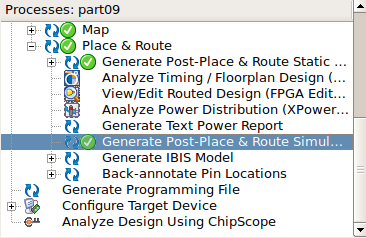
\includegraphics[width=1\textwidth]{proof.png}
            \caption{Successful Post-Place \& Route Simulation} \label{fig:proof}
        \end{center}
    \end{figure}

    The module and its test bench with explicit port declarations and a 50 MHz clock were synthesized, and the waveforms were generated.

    \begin{figure}[ht]
        \begin{center}
            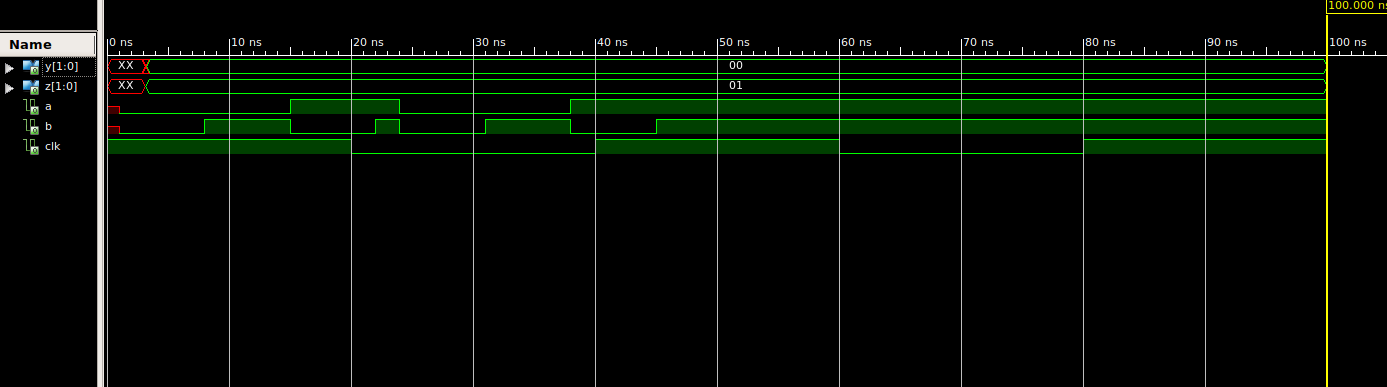
\includegraphics[width=1\textwidth]{wav.png}
            \caption{Waveform Generated from Part 9 Test Bench} \label{fig:wav}
        \end{center}
    \end{figure}

    The output from the test bench were saved in the following table:

    \begin{table}[h]

        \caption{Inputs and Outputs of The Part 9 Test Bench}
        \centering
        \begin{tabular*}{200pt}{@{\extracolsep{\fill}} ccccc}

            \textbf{time} & \textbf{a} & \textbf{b} & \textbf{y} & \textbf{z} \\
            \hline
            3000 & 0 & 0 & xx & xx \\
            3000 & 0 & 0 & 0x & 01 \\
            3000 & 0 & 0 & 00 & 01 \\
            8000 & 0 & 1 & 00 & 01 \\
            10000 & 0 & 1 & 00 & 01 \\
            15000 & 1 & 0 & 00 & 01 \\
            17000 & 1 & 0 & 00 & 01 \\
            22000 & 1 & 1 & 00 & 01 \\
            24000 & 0 & 0 & 00 & 01 \\
            26000 & 0 & 0 & 00 & 01 \\
            31000 & 0 & 1 & 00 & 01 \\
            33000 & 0 & 1 & 00 & 01 \\
            38000 & 1 & 0 & 00 & 01 \\
            40000 & 1 & 0 & 00 & 01 \\
            45000 & 1 & 1 & 00 & 01 \\
            47000 & 1 & 1 & 00 & 01 \\

        \end{tabular*}
    \end{table}


    \section{Observations}
    The outputs do not appear to be affected after the post-synthesis. In the presynthesis simulations, the test bench would display changes on the outputs. The post-synthesis simulation appears to only affect after the initial change in the clock. The lack of expected changes in the outputs may be caused due to the improper implementation in the original module.

\end{document}
